% !TeX root = ../bbchallenge-paper.tex

\subsection{Loops}\label{sec:loops}
\subsubsection{Loop-detection algorithm}
\begin{figure}[h!]
  \centering
  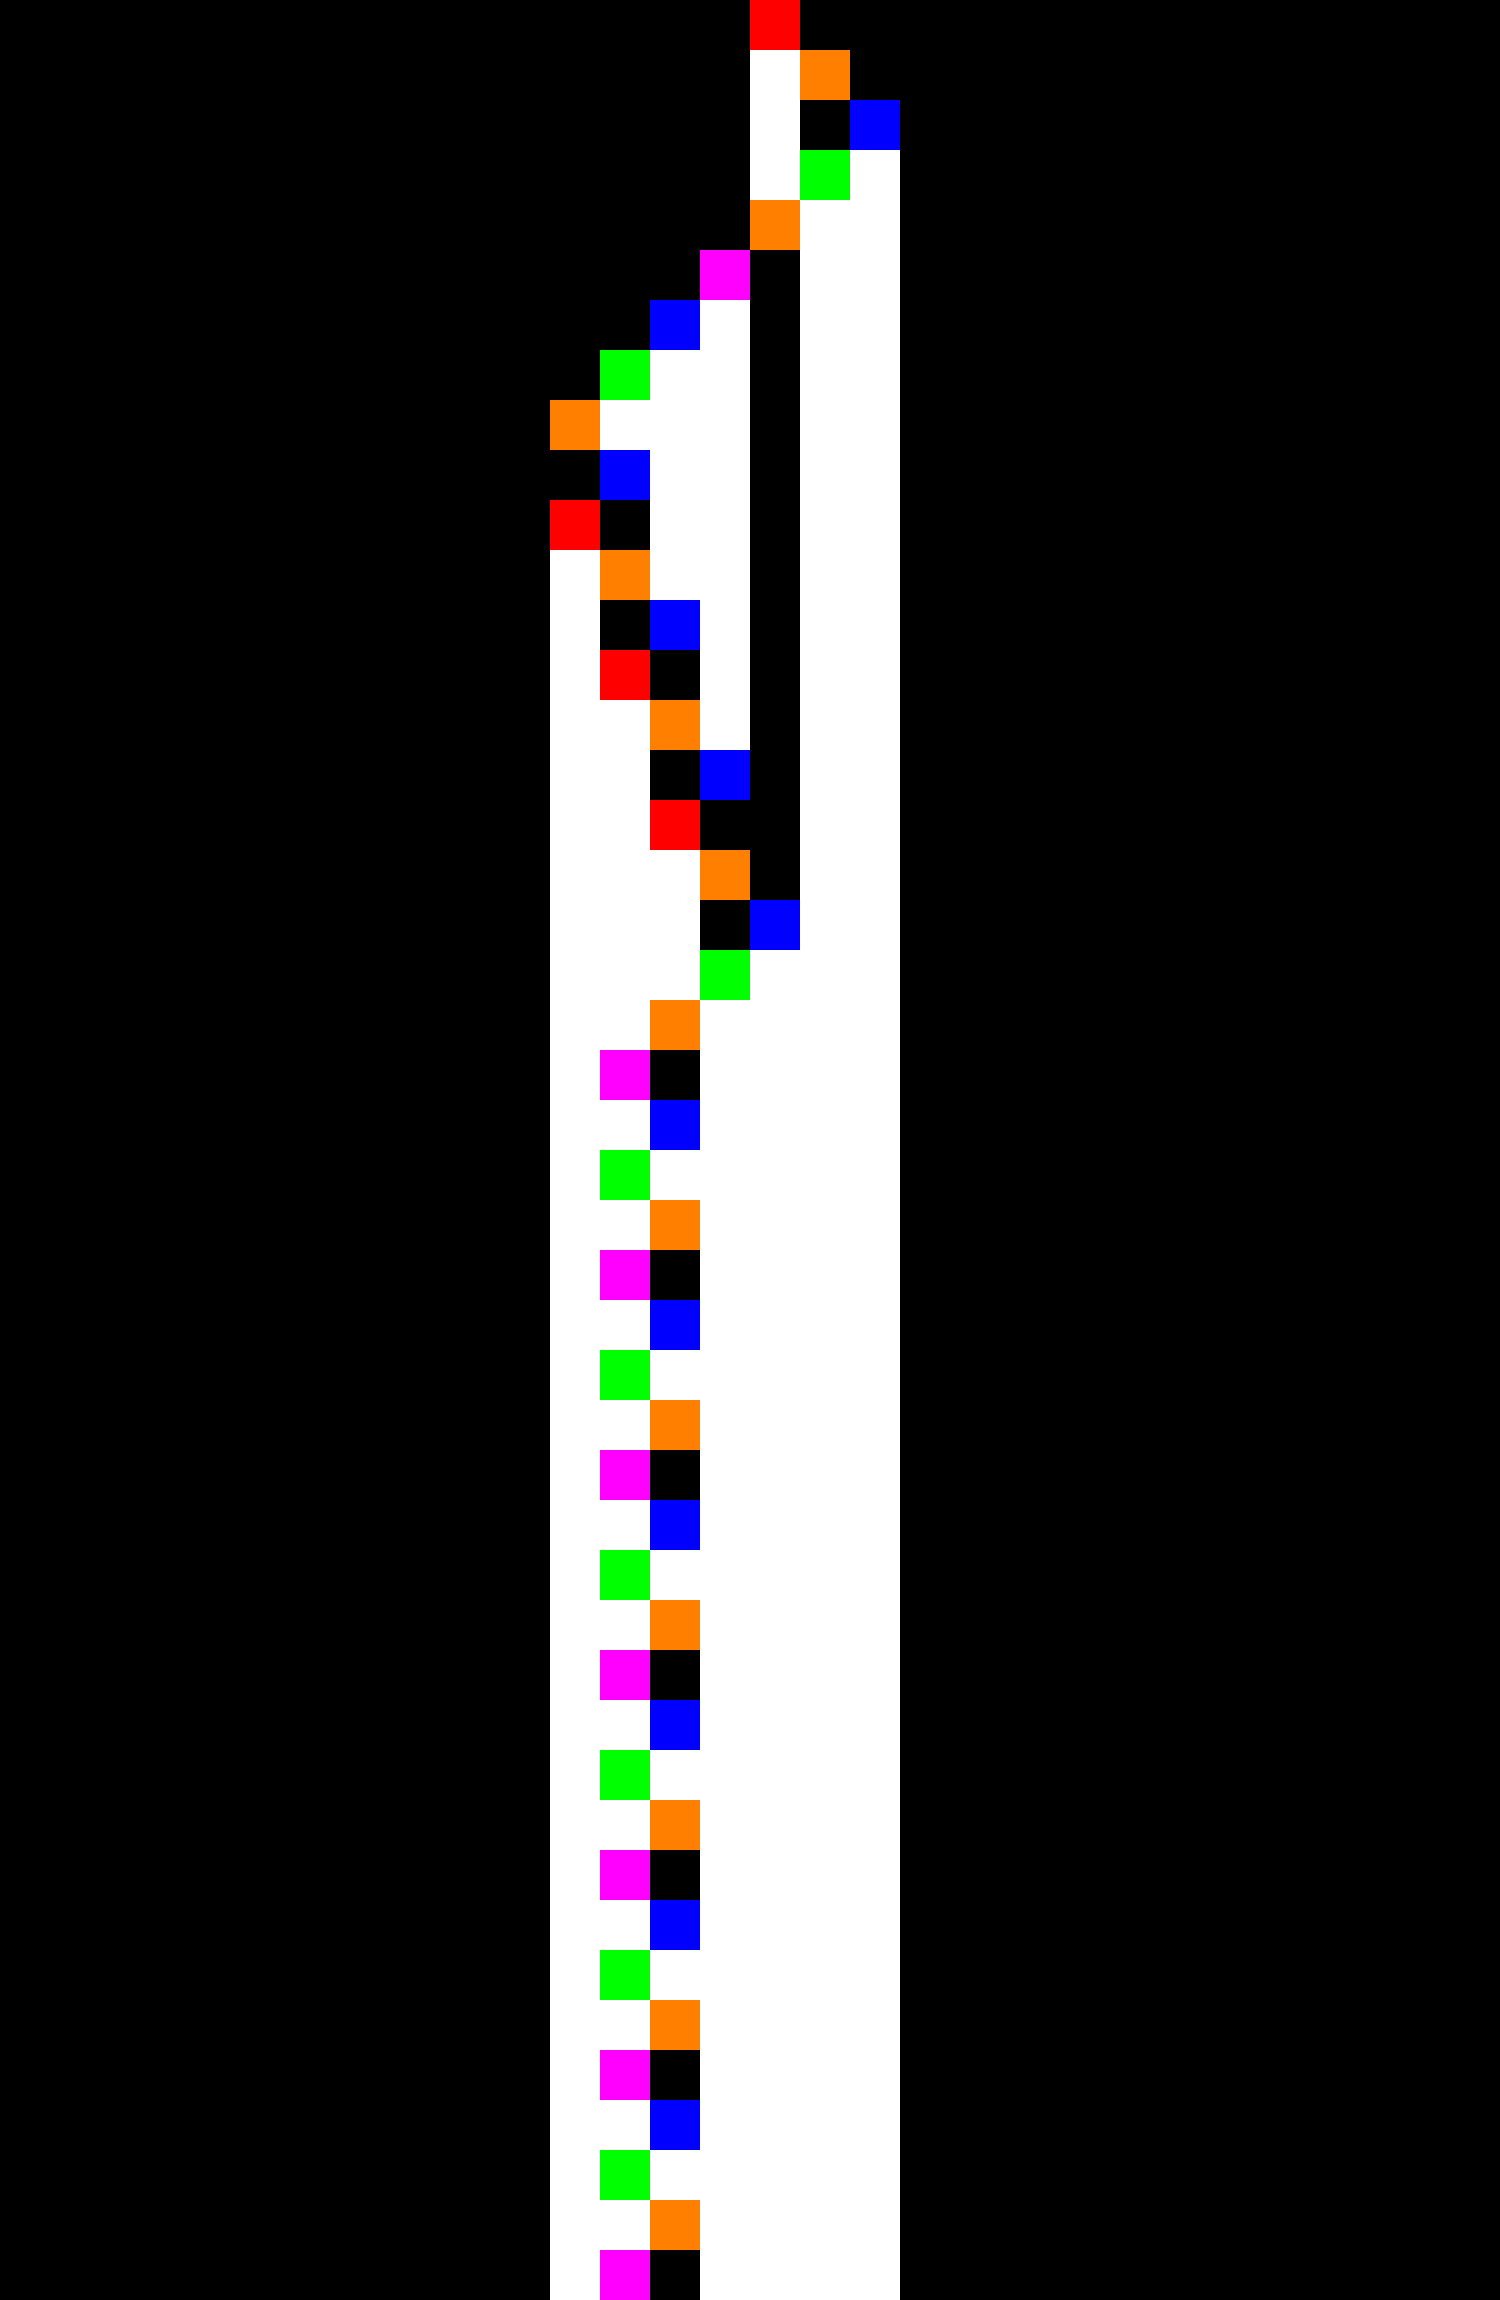
\includegraphics[width=0.4\textwidth]{figures/space-time-diagrams/cycler_279081.pdf}
  \hspace{2ex}
  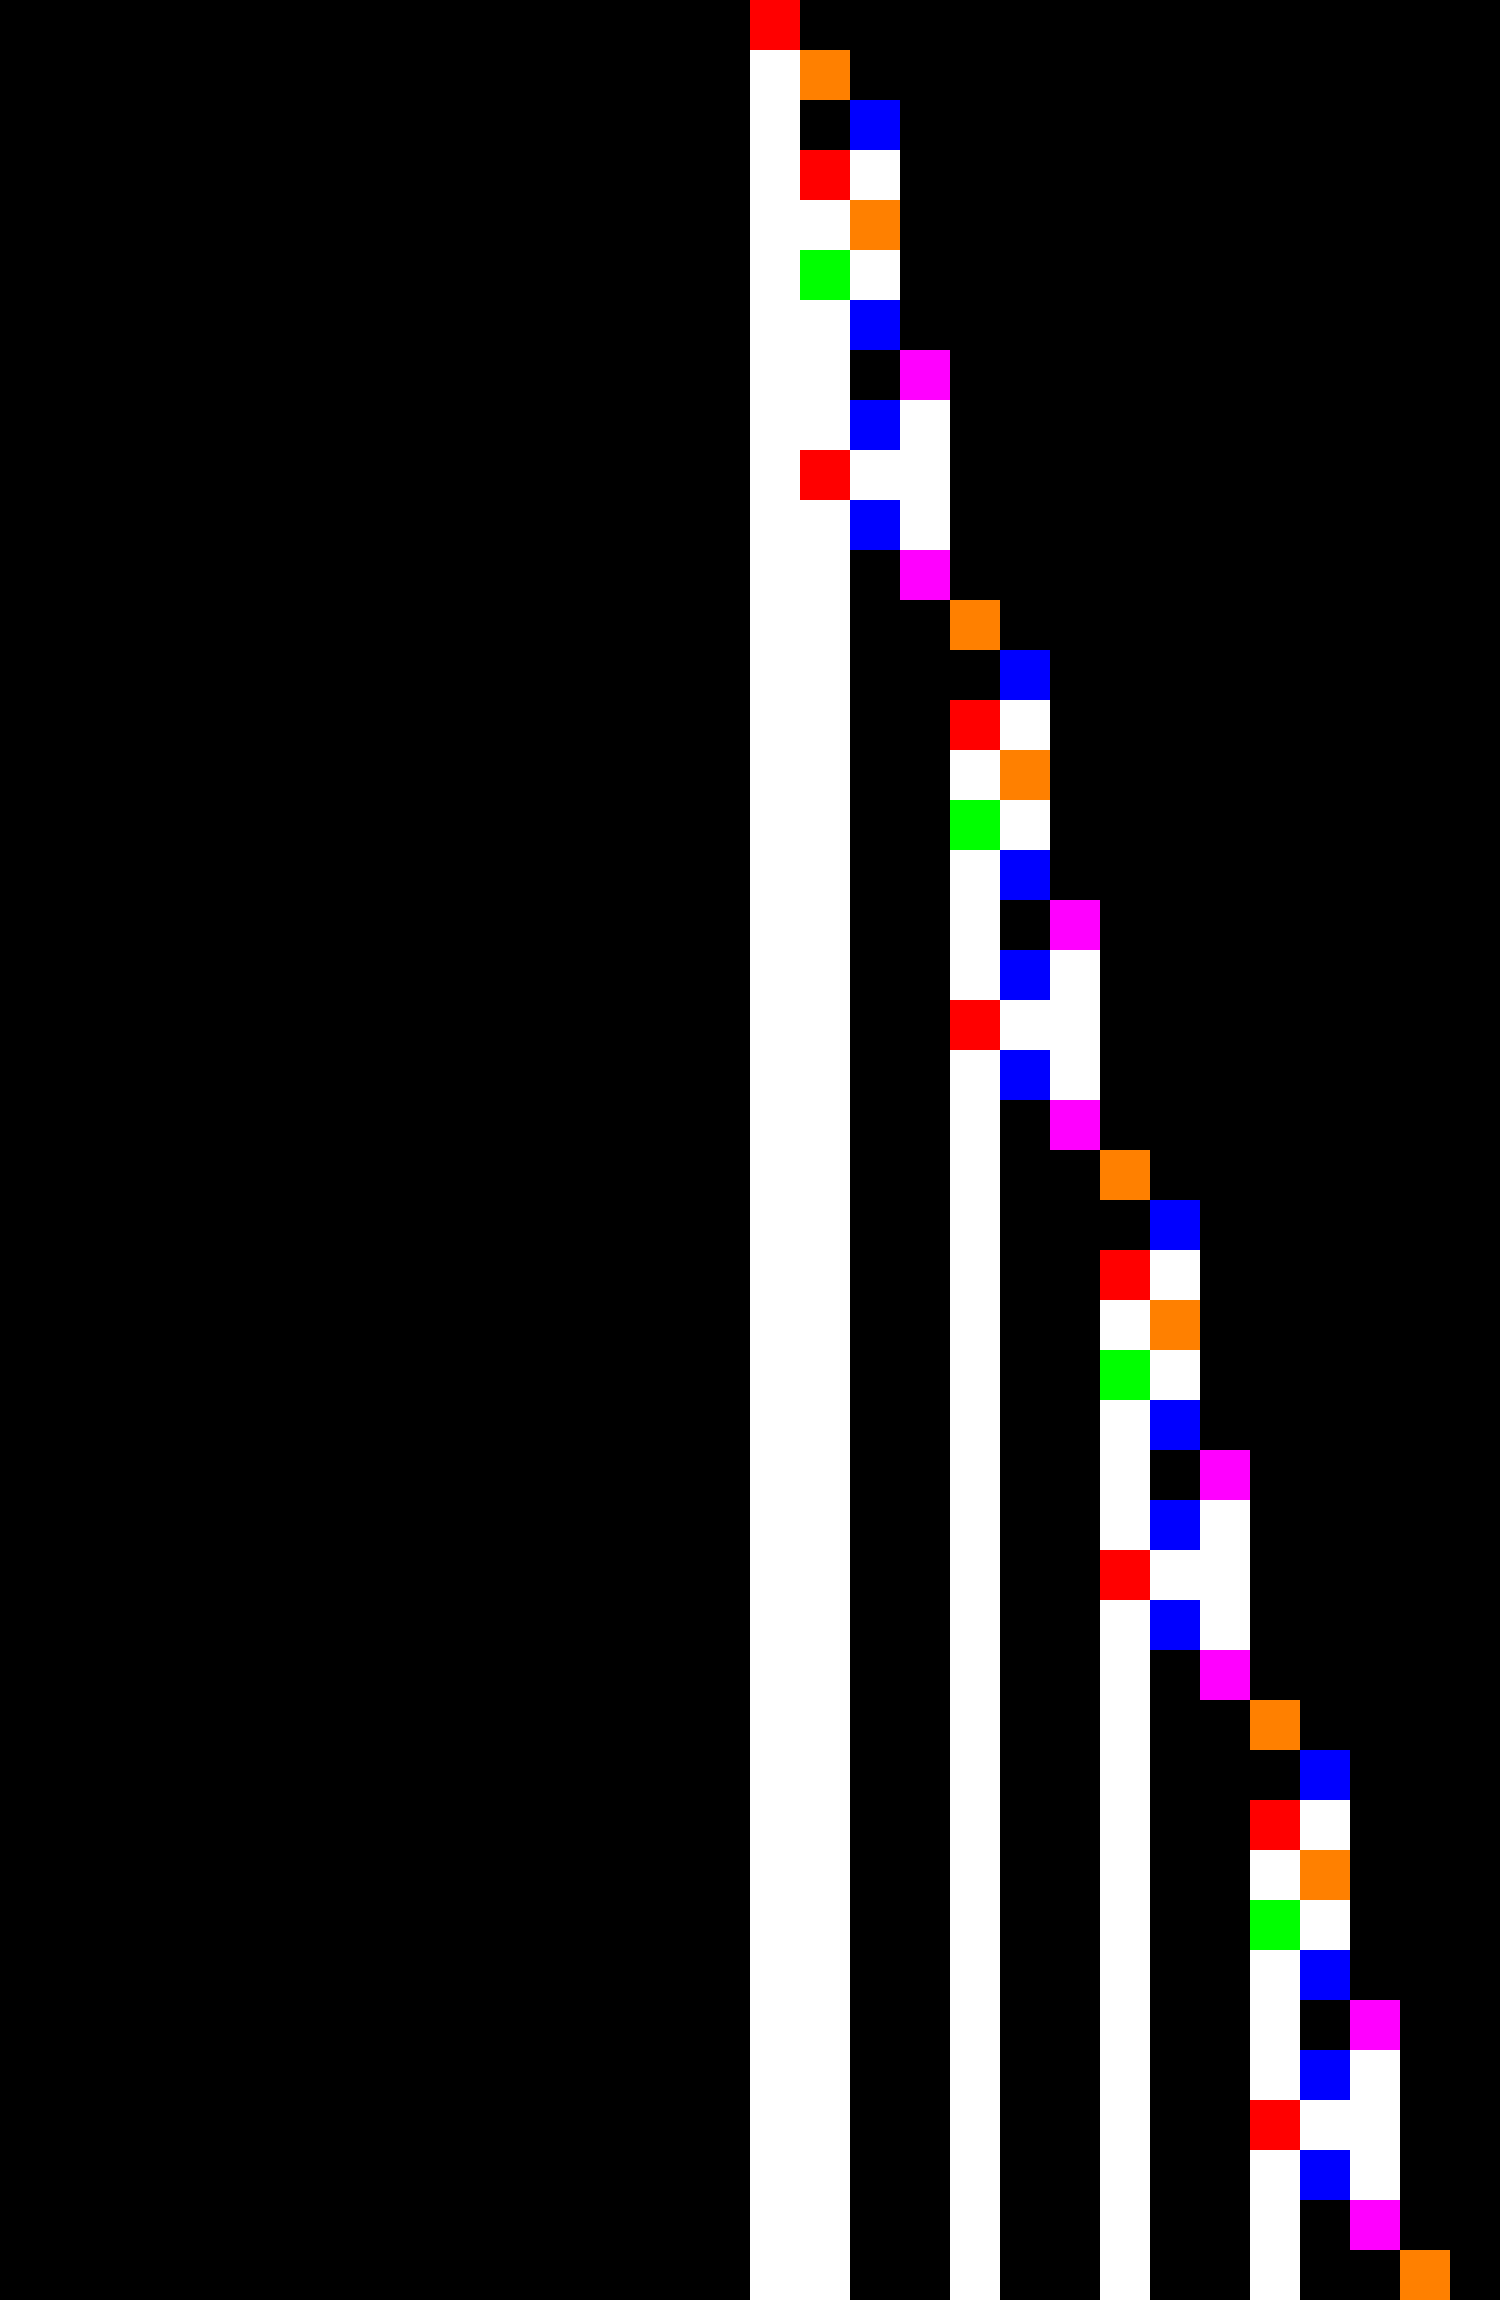
\includegraphics[width=0.4\textwidth]{figures/space-time-diagrams/translated_cycler_62645534.pdf}
  %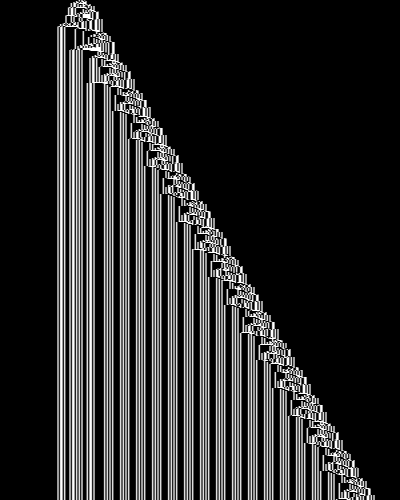
\includegraphics[width=0.4\textwidth]{figures/space-time-diagrams/translated_cycler_59090563_2.png}
  \caption{Space-time diagrams of the 30 first steps of a \textit{\cycler}\protect\footnotemark  with colors indicating head position and state: \stateA, \stateB, \stateC, \stateD, \stateE (left) and of the 10,000 first steps of a \textit{\TC}\protect\footnotemark (right). \cyclers are machines that eventually repeat the same configuration forever. \TCs are machines that eventually repeats the same configuration forever, but translated in space. We refer to these two types of machines as \textit{loops}.}\label{fig:loops}
\end{figure}

\footnotetext{\url{https://bbchallenge.org/1RB---\_0RC0LE\_1LD0LA\_1LB1RB\_1LC1RC}}
\footnotetext{\url{https://bbchallenge.org/1RB0RE\_0LC1RC\_0RD1LA\_1LE---\_1LB1RC}}

The goal of this decider is to recognise two types of Turing machines: (i) \textit{\cyclers} (see Figure~\ref{fig:loops}~left) that eventually repeat the same configuration and therefore loop forever and (ii) \textit{\TCs} that also eventually repeat the same configuration, but translated in space (see Figure~\ref{fig:loops}~right). We regroup both types of machines under the umbrella term of \textit{loops}.

Deciding Cyclers reduces to the well-known mathematical problem of detecting the cycles of a function and standard detection algorithms exist \cite{wiki:Cycle_detection}, the simplest one consisting in memorizing each successive configuration of the machine until encountering one that has been already seen. Translated Cyclers, also known as \textit{Lin's recurrence}, have first been described and decided in Shen Lin's 1963 PhD thesis \cite{Lin1963}, other algorithms to detect them have been developed since then\footnote{\url{https://discuss.bbchallenge.org/t/decider-translated-cyclers/34}}.

Here, we develop a new algorithm (Algorithm~\ref{alg:loops}) for deciding both \cyclers and \TCs. The particularity of this algorithm is that it detects loops only by analysing the history of state, read-symbol and \headposs visited by the machine, instead of considering entire configurations (\ie with full tape content information).

Let's call the \textit{transcript} of a machine the list of successive \ssps visited by the machine from the all-zero tape. For instance, the transcript of the \cycler in Figure~\ref{fig:loops}~(left) starts with \texttt{A0 B0 C0 D0 B1 E0 C0 D0 B0 C1 A0} and the transcript of the \TC in Figure~\ref{fig:loops}~(right) starts with \texttt{A0 B0 C0 A0 B1 D1 C1 E0 C0 A1 C1}. Surprisingly, it turns out that in order to detect loops, we only have to track when a transcript repeats the same sequence twice back-to-back, for instance, in the case of the Cycler in Figure~\ref{fig:loops}: \texttt{A0 B0 C0 D0 B1 E0 C0 D0 B0 C1 A0 B0 C1 A0 B0 C1 A0 B0 C0 D0 \textbf{\underline{B1 E1 C0 D1}} \textbf{\underline{B1 E1 C0 D1}}}. When such a repetition occurs, we use the extra information of \headpos to conclude:

\begin{itemize}
  \item if when entering the second repetition the head is at the same position it was at the beginning of the first repetition, then we have detected a \cycler, \eg for the \cycler in Figure~\ref{fig:loops}~(left), here is the end of the transcript with extra head-position information given after each \ssp: \texttt{\underline{\textbf{B1(-2)} E1(-3) C0(-2) D1(-3)} \underline{\textbf{B1(-2)} E1(-3) C0(-2) D1(-3)}}.

  \item if each time that the \headpos attains a local extremum (\ie a position that is strictly bigger or smaller than any previously seen position, also known as \textit{record-breaking}) in either repetition, it also corresponds to a local extremum in the other repetition, then we have detected a \TC, \eg for the \TC in Figure~\ref{fig:loops}~(right), the transcript (with \headpos information) is: \texttt{A0(0) \underline{B0(1)* C0(2)* A0(1) B1(2) D1(1) C1(2) E0(3)* C0(2) A1(1) C1(2) E1(3)} \\ \underline{B0(4)* C0(5)* A0(4) B1(5) D1(4) C1(5) E0(6)* C0(5) A1(4) C1(5) E1(6)}} etc., with all record-breaking positions marked \texttt{*} in the repeated \ssp pattern \texttt{B0 C0 A0 B1 D1 C1 E0 C0 A1 C1 E1}.

\end{itemize}

This logic is encoded in Algorithm~\ref{alg:loops}, l.\ref{alg:loops:test} and we prove that this algorithm is correct in Theorem~\ref{th:loops}.

\begin{theorem}[Coq-BB5: \texttt{Lemma loop1\_decider\_WF}]\label{th:loops}
  Let $\mathcal{M}$ be a Turing machine and $L \in \N^+$ a step-limit. \textsc{decider-loops}($\mathcal{M}$, $L$) terminates and its result is correct -- see Algorithm~\ref{alg:loops}:
  \begin{itemize}
    \item If the result is \texttt{HALT} then $\mathcal{M}$ halts from the all-zero tape.
    \item If the result is \texttt{NONHALT} then $\mathcal{M}$ does not halt from the all-zero tape.
  \end{itemize}
\end{theorem}
\begin{proof}
  The call to \textsc{decider-loops}($\mathcal{M}$, $L$) terminates because of Algorithm~\ref{alg:loops}, l.\ref{alg:loops:terminate}. The call returns \texttt{HALT} if and only if $\mathcal{M}$ halts within $L$ steps from the all-zero tape, see Algorithm~\ref{alg:loops}, l.\ref{alg:loops:halt}, hence if the call returns \texttt{HALT} we know that the machine halts. The interesting case is the loop-detection leading to \texttt{NONHALT}. We leave this case as an exercise for the reader.

  % We take the same terminology than Algorithm~\ref{alg:loops}: $h_i = (s_i,m_i,d_i) \in \states \times \alphabet \times \Z$ for $0 \leq i \leq L$ correspond the successive state, read-symbol and tape position reached. Let's assume the algorithm returns \texttt{NONHALT} for some loop length parameter $l \geq 0$: we have $s_{L-i} = s_{K-i}$ and $m_{L-i} = m_{K-i}$ for all $i \in [0,l]$ with $K = L-l-1$ and each $h_{L-i}$ is \textit{record-breaking} (\ie \headpos that is strictly bigger or smaller than any previously seen \headpos) iff $h_{K-i}$ is. Algorithm~\ref{alg:loops}, l.\ref{alg:loops:test} distinguishes two cases:

  % \begin{enumerate}
  %   \item $d_L$ is equal to $d_K$. In that case, let's show that $h_{L+1}$ is defined and that $h_{L+1} = h_{K+1}$. Because $s_K = s_L$ and $m_K = m_L$, the machine is in same state and reads same symbol at steps $K$ and $L$, hence the same transition is applied to go from $h_K$ to $h_{K+1}$ than from $h_L$ to $h_{L+1}$, meaning that $s_{L+1} = s_{K+1}$; furthermore, because $d_L = d_{K}$ we have $d_{L+1} = d_{K+1}$. Hence, $h_{L+1}$ is defined (\ie the machine has not halted), but it remains to prove that the read-symbol is the same, \ie $m_{L+1} = m_{K+1}$. First, let's notice than by the same argument we can conclude that $d_{L-i} = d_{K-i}$ for all $i \in [0,l]$. Then, let's consider $i_0 = \text{max}\{i \, | \, d_i = d_{K+1},\, i < L+1\}$. We know that $i_0$ is defined since $i_0 \geq K+1$. Piecing together what we know, we have that $h_{i_0} = h_{i_0 -l - 1}$ and therefore that $m_{L+1} = m_{K+1}$ since there is no step between $i_0$ and $L+1$ where position $d_{L+1}$ is reached, as well as no step between $i_0-l-1$ and $K+1$ where $d_{K+1} = d_{L+1}$ is reached, and the same transition was taken at $h_{i_0} = h_{i_0 -l - 1}$. Hence, $h_{L+1} = h_{K+1}$. Using this reasoning as induction step shows that, for all $i \in \N$ and $i' = i \text{ mod } l+1$, we have $h_{L+i} = h_{K+i'}$. The transcript of $\mathcal{M}$ is infinite, the machine does not halt from the all-zero tape.
  %   \item $d_L$ is not equal to $d_K$ but \headpos records were broken. Let's slightly modify $h_i$ to be $h_i = (s_i,m_i,b_i) \in \states \times \alphabet \times \mathbb{B}$ where $b_i$ being \texttt{true} iff $d_i$ broke a record (\ie if for all $0 \geq j < i$ we have $d_j < d_i$). We know that $h_{L-i} = h_{K-i}$ for all $i \in [0,l]$. Let's show that $h_{L+1}$ is defined and that $h_{L+1} = h_{K+1}$. Similarly as in the first case, because $s_K = s_L$ and $m_K = m_L$ we know that $h_{L+1}$ is defined and $s_{L+1} = s_{K+1}$. Two cases:
  %         \begin{itemize}
  %           \item If $h_{K}$ and $h_{L}$ are record-breaking. If $h_{K+1}$ is record-breaking then so is $h_{L+1}$ because the head move direction is the same from $h_{K}$ to $h_{K+1}$ and $h_{L}$ to $h_{L+1}$. Hence, $m_{L+1} = m_{K+1} = 0$ and we have  $h_{L+1} = h_{K+1}$. If $h_{K+1}$ is not record-breaking, then $h_{L+1}$ is not record-breaking either again because head move directions are the same. In that case, because the cell at position $d_{L+1}$ has already been seen, we can apply the same argument as in case 1 above ($d_L = d_K$) and conclude that $h_{L+1} = h_{K+1}$.
  %           \item If $h_{K}$ and $h_{L}$ are not record-breaking. If $h_{K+1}$ is record-breaking then so is $h_{L+1}$. \ts{TS: TO FINISH}
  %         \end{itemize}


  % \end{enumerate}

\end{proof}


\begin{algorithm}
  \caption{{\sc decider-Loops}, reformulates the algorithm \texttt{loop1\_decider} of Coq-BB5.}\label{alg:loops}

  \begin{algorithmic}[1]
    \State{\textbf{Input:} A Turing machine `$\mathcal{M}$', a step-limit parameter $L$.}
    \State{\textbf{Output:} `NONHALT' if the decider detects that the machine is a loop, `HALT' if the machine halts and `UNKNOWN' otherwise.}

    \State
    \State Simulate $\mathcal{M}$ for $L$ steps and save the history of each consecutive state, read-symbol and tape position reached, \ie consecutive $h_i = (s_i,m_i,d_i)\in\states\times\alphabet\times\Z$ for $0 \leq i \leq L$ and $h_0 = (\stateA,\symbolzero,0)$.


    \State \If{the machine has halted before $L$ steps}
    \State \Return HALT \label{alg:loops:halt}
    \EndIf
    \State \For{$l$ \textbf{in} $[0,+\infty[$ } \Comment{$l+1$ is the length of the potential loop}
    \State \If{$2(l + 1) > L$} \Comment{The history does not contain two potential loops of size $l+1$}
    \State \Return UNKNOWN \label{alg:loops:terminate}
    \State \EndIf
    \State $K = L-l-1$
    \State $\text{allequal} = \text{true}$
    \State $\text{recordbreak} = \text{false}$
    \State \For{$i$ \textbf{in} $[0,l]$ } \Comment{Comparing \ssp equality at each step of both potential loops}
    \State $s,m,d = h_{L-i}$
    \State $s',m',d' = h_{K-i}$
    \State
    \State $\text{recordbreak1} = \text{false}$
    \State $\text{recordbreak2} = \text{false}$
    \State \If{$s\neq s'$ \textbf{or} $m \neq m'$}
    \State $\text{allequal} = \text{false}$
    \State \textbf{break}
    \EndIf
    \State \If{$d > \text{max} \{d_j \, | \, j < L-i \}$ \textbf{or} $d < \text{min} \{d_j \, | \, j < L-i \}$}
    \State $\text{recordbreak1} = \text{true}$
    \State $\text{recordbreak} = \text{true}$
    \EndIf
    \State \If{$d' > \text{max} \{d'_j \, | \, j < K-i \}$ \textbf{or} $d' < \text{min} \{d'_j \, | \, j < K-i \}$}
    \State $\text{recordbreak2} = \text{true}$
    \EndIf
    \State \If{$\text{recordbreak1} \neq \text{recordbreak2}$}
    \State $\text{allequal} = \text{false}$
    \State \textbf{break}
    \EndIf
    \EndFor
    \State \If{$\text{allequal}$ \textbf{and} ($d_L == d_K$ \textbf{or} $\text{recordbreak}$)}\label{alg:loops:test}
    \State \Return NONHALT
    \EndIf
    \EndFor

  \end{algorithmic}

\end{algorithm}

\subsubsection{Loops: results}\label{sec:loops:results}

\begin{table}[h!]
  \centering
  \begin{tabular}{llll}
    Step-limit parameter $L$ & Nonhalt                         & Halt                           & Total decided \\
    130                      & 126,950,828                     & 48,367,435                     & 175,318,263   \\
    4100                     & 43,269                          & 12,276                         & 55,545        \\
    1,050,000                & 2                               & 0                              & 2             \\ \hline
    Total                    & \multicolumn{1}{r}{126,994,099} & \multicolumn{1}{r}{48,379,711} & 175,373,810
  \end{tabular}
  \caption{5-state machines decided by loops (Algorithm~\ref{alg:loops}) per step-limit parameter $L$.}\label{tab:paramsLoops}
\end{table}

Algorithm~\ref{alg:loops} is implemented as part of Coq-BB5 (function \texttt{loop1\_decider}). As advertised in the $S(5)$ pipeline (Table~\ref{tab:pipelineBB5}), the decider for loops decides a very important proportion the enumerated 5-state Turing machines: 95.48\% of the nonhalting machines and 99.99\% of the halting ones and this with fairly low step-limit parameters, see Table~\ref{tab:paramsLoops}! This means, for instance, that 99.99\% of the enumerated 5-state halting machines halt before $4,100$ steps.